\documentclass[a4paper]{article}

\usepackage[english]{babel}
\usepackage[utf8x]{inputenc}
\usepackage{amsmath}
\usepackage{graphicx}
\usepackage[colorinlistoftodos]{todonotes}
\usepackage{fullpage}
\usepackage{amsfonts}
\usepackage{hyperref}
\usepackage{url}
\usepackage{pdfpages}
\usepackage{comment}

\title{Report of Project: Build an Adversarial Game Playing Agent}
\author{Israel G. de Oliveira}
\date{January 27, 2019}
\begin{document}
\maketitle

\section{Introduction}
This report is about the building an adversarial game playing agent, project part from Artificial Intelligence Nanodegree \cite{githubUdacityAIND}. The objective is implement a agent to play Isolation versus the others 3 sample agents (players): the first agent chooses randomly the next move, the second agent uses Greedy Search and the third uses Minimax Search. The isolation game for this project uses as token the knight in chess, with L-shaped movements \cite{githubUdacityAINDProj3}. This project is based on book Artificial intelligence: a modern approach \cite{russell2009artificial}.

\subsection{Heuristics}

The option choosen was 'Option 1': Develop a custom heuristic (must not be one of the heuristics from lectures, and cannot only be a combination of the number of liberties available to each agent). For this report, it is implemented the Minimax with $\alpha\beta$-pruning (MM-$\alpha\beta$) \cite{elnaggar2014comparative} search method with two different strategies, 8 ways of calculating score. Totalizing 16 different heuristics.

\begin{itemize}
    \item Search strategy 1: move to $X_{own} = S_1(G_s)$, with actual play $c_{play}$, MM-$\alpha\beta (G_s,d)$, game state $G_s$, depth $d$
    
    \begin{equation}
        S_1(G_s) = \left \{
        \begin{matrix} 
        57 &  c_{play} < 3,~ X_{opp} \neq 57 \\
        0 &  c_{play} < 3,~ X_{opp} = 57 \\
        \text{MM-$\alpha\beta$}(G_s,2) & c_{play} \in [3, 9] \\
        \text{MM-$\alpha\beta$} \left ( G_s, 1+\left \lfloor \frac{c_{play}}{10} \right \rfloor \right ) & c_{play} > 9
        \end{matrix} \right .
        \label{S1}
    \end{equation}
    
    In first two plays, the ideia is choose the center ($57$) or the corner ($0$). One is a classical strategic start, the other is the furthest from the opponent position (if this position is the center). For next first 9 moves, it is not interesting search deeper for a solution, just evolve the game keeping good positions. For the last moves (more than 9 plays), it is interesting search more deeper as the game evolve. When the game comes to end, the game tree is shorter, so it is possible to go deep in the tree to achieve the better strategy possible without less computing time.
    
        \item Search strategy 2:
    
    \begin{equation}
        S_2(G_s) = \left \{
        \begin{matrix} 
        57 &  c_{play} < 3,~ X_{opp} \neq 57 \\
        5 &  c_{play} < 3,~ X_{opp} = 5 \\
        \text{MM-$\alpha\beta$}(G_s,2) & c_{play} \in [3, 6] \\
        \text{MM-$\alpha\beta$} \left ( G_s, \max \left ( \left \lfloor \frac{c_{play}}{10} \right \rfloor, 3 \right ) \right ) & c_{play} > 6
        \end{matrix} \right .
        \label{S2}
        \end{equation}
Similar to the first strategy, but going in a little more deeper in the beginning of the game. The idea is check if going deeper is better (more wins).
    
    \item Score heuristic 1: the score function chosen is based in how much legal moves each player have (liberties), $L_{own}$ and $L_{opp}$. 
    
    \begin{equation}
        \text{SH}_1(G_s) = C_1(G_s)  L_{own} - C_2(G_s) L_{opp}  \label{SH1}
    \end{equation}
    
    \noindent with $C_i(\cdot)$ achieved with other functions, wich will be discussed after. The main idea with this score function is consider the liberty of the oppenent, e.g. if possible to consider a victory move when this zero they amount os moves. With different strategies for achieve $C_i(\cdot)$, cahges the behavior of this searching for the best move.
    
    \item Score heuristic 2: 
    
    \begin{equation}
        \text{SH}_1(G_s) =  \frac{C_4(G_s)}{C_2(G_s) L_{opp} + \varepsilon} - \frac{C_3(G_s)}{C_1(G_s) L_{own} + \varepsilon}  \label{SH2}
    \end{equation}
    
    \noindent with $\varepsilon = 10^{-10}$. The main idea is accentuate the difference between liberties, when one have much more liberties then other, it will pointed out. With the experiments, it is possible to check how better this score function is.
    
    \item Calculation of weights 1: this is how calculate the functions $C_i(\cdot)$.
    
    \begin{equation}
        C(G_s) =  \begin{bmatrix} 1 \\ 1 \\ 4 \\ 4 \end{bmatrix}  \label{C1}
    \end{equation}
    
    \noindent Constants, for any game state.
    
    \item Calculation of weights 2:
    
    \begin{equation}
        C(G_s) =  \begin{bmatrix} 
        1/2+1/({2+c_{play}}) \\
        3/2-1/({2+c_{play}}) \\ 
                                  4 \\ 4 \end{bmatrix}  \label{C2}
    \end{equation}
    
    \noindent This way it is possible to improve the focus on knocking down the opponent with the passing of the game. Changing the focus gradually during the game.
    
    \begin{eqnarray}
        C_1(\cdot) &\in& [1, 0.5) \\
        C_2(\cdot) &\in& [1, 1.5) 
    \end{eqnarray}
    
    \item Calculation of weights 3: 
    
    \begin{equation}
        C(G_s) =  \begin{bmatrix} 
        1+8/({1+c_{play}}) \\
        8-8/({1+2c_{play}}) \\ 
                                  6 \\ 6 \end{bmatrix}  \label{C3}
    \end{equation}
    
    \noindent Similar to second, but with more intense variation.
    
    \begin{eqnarray}
        C_1(\cdot) &\in& [9, 1) \\
        C_2(\cdot) &\in& [0, 8) 
    \end{eqnarray}
    
    \item Calculation of weights 4:
     
    \begin{equation}
        C(G_s) =  \begin{bmatrix} 
        1+2/({1+c_{play}}) \\
        3-2/({1+2c_{play}}) \\ 
                                  6 \\ 6 \end{bmatrix}  \label{C4}
    \end{equation}
    
    \noindent Similar to third, but with different limit values.
    
    \begin{eqnarray}
        C_1(\cdot) &\in& [3, 1) \\
        C_2(\cdot) &\in& [1, 3) 
    \end{eqnarray}
    
\end{itemize}

\section{Experiments}

Combining the two search stategies (\ref{S1}) and (\ref{S2}), the two heuristics scores (\ref{SH1}) and (\ref{SH2}) and four ways to calculate the constants, we achive 16 agents. Falowing the tag: S$a$SC$b$W$c$, with $a$ the number of the search strategy, $b$ the number of the heuristic score and $c$ the number of the function to calculate the constants. The whole experiment is composed by: 100 rounds, with fair matches, totaling 400 matches. The time limit for give a move is 150 ms, default in the framework provided by Udacity.

\subsection{Results}

\begin{figure}[htpb]
\begin{center}
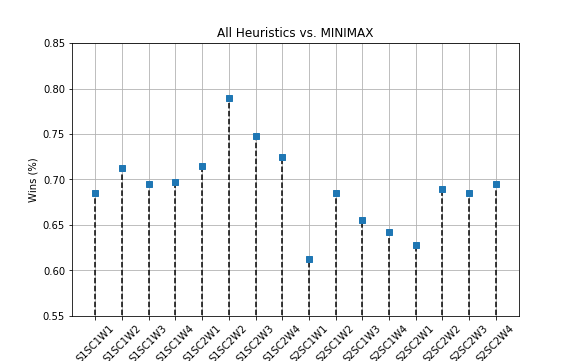
\includegraphics[width=1\columnwidth]{fig/results_Wins_All_vs_MINIMAX.png}
\caption{Wins for all custom heuristics vs. sample player MINIMAX.}
\end{center}
\label{figwinsMINIMAX}
\end{figure}
    

    \begin{table}[htpb]
    \caption{ Wins: all custom heuristics vs. sample player MINIMAX.}
    \centering
    \begin{tabular}{ l | c }
    Heuristic & Wins (\%) \\ \hline 
    S1SC1W1 & 0.685 \\
    S1SC1W2 & 0.7125 \\
    S1SC1W3 & 0.695 \\
    S1SC1W4 & 0.6975 \\
    S1SC2W1 & 0.715 \\
    S1SC2W2 & 0.\textbf{79} \\
    S1SC2W3 & 0.7475 \\
    S1SC2W4 & 0.725 \\
    S2SC1W1 & 0.6125 \\
    S2SC1W2 & 0.685 \\
    S2SC1W3 & 0.655 \\
    S2SC1W4 & 0.6425 \\
    S2SC2W1 & 0.6275 \\
    S2SC2W2 & 0.69 \\
    S2SC2W3 & 0.685 \\
    S2SC2W4 & 0.695 
    \end{tabular}
    \label{tabwinsMINIMAX}
    \end{table}


In figure \ref{figwinsMINIMAX} and table \ref{tabwinsMINIMAX}, all methods vs. MINIMAX, it is possible to see a improvement with the proposed heuristics. The first search strategy (\ref{S1}) achieve better results then (\ref{S2}), independent of all score heuristics. With search strategy (\ref{S1}), the wins is around 70\%, a sginificant improvement. Looking only for the scores (\ref{SH1}) and (\ref{SH2}), the second appears to be better. For weights, the (\ref{C2}) has a prominence among the others.
    
%==============================================


\begin{figure}[htpb]
\begin{center}
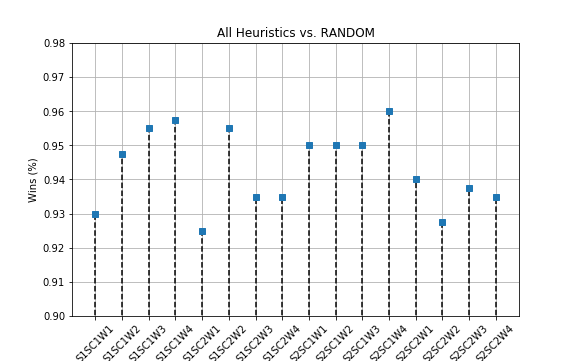
\includegraphics[width=1\columnwidth]{fig/results_Wins_All_vs_RANDOM.png}
\caption{Wins for all custom heuristics vs. sample player RANDOM.}
\end{center}
\label{figwinsRANDOM}
\end{figure}
    

    \begin{table}[htpb]
    \caption{ Wins: all custom heuristics vs. sample player RANDOM.}
    \centering
    \begin{tabular}{ l | c }
    Heuristic & Wins (\%) \\ \hline 
    S1SC1W1 & 0.93 \\
    S1SC1W2 & 0.9475 \\
    S1SC1W3 & 0.955 \\
    S1SC1W4 & 0.9575 \\
    S1SC2W1 & 0.925 \\
    S1SC2W2 & 0.955 \\
    S1SC2W3 & 0.935 \\
    S1SC2W4 & 0.935 \\
    S2SC1W1 & 0.95 \\
    S2SC1W2 & 0.95 \\
    S2SC1W3 & 0.95 \\
    S2SC1W4 & \textbf{0.96} \\
    S2SC2W1 & 0.94 \\
    S2SC2W2 & 0.9275 \\
    S2SC2W3 & 0.9375 \\
    S2SC2W4 & 0.935 
    \end{tabular}
    \label{tabwinsRANDOM}
    \end{table}

In figure \ref{figwinsRANDOM} and table \ref{tabwinsRANDOM} vs. a Player Agent using randomly moves, it is possible to see great improvement with the proposed heuristics. However, it is not possible to infer something relevant about the search strategies and heuristics: appears have not a pattern throw the methods.

    
%==============================================


\begin{figure}[htpb]
\begin{center}
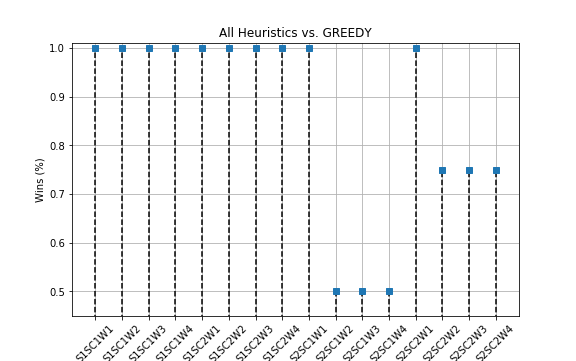
\includegraphics[width=1\columnwidth]{fig/results_Wins_All_vs_GREEDY.png}
\caption{Wins for all custom heuristics vs. sample player GREEDY.}
\end{center}
\label{figwinsGREEDY}
\end{figure}
    

    \begin{table}[htpb]
    \caption{ Wins: all custom heuristics vs. sample player GREEDY.}
    \centering
    \begin{tabular}{ l | c }
    Heuristic & Wins (\%) \\ \hline 
    S1SC1W1 & \textbf{1.0} \\
    S1SC1W2 & \textbf{1.0} \\
    S1SC1W3 & \textbf{1.0} \\
    S1SC1W4 & \textbf{1.0} \\
    S1SC2W1 & \textbf{1.0} \\
    S1SC2W2 & \textbf{1.0} \\
    S1SC2W3 & \textbf{1.0} \\
    S1SC2W4 & \textbf{1.0} \\
    S2SC1W1 & \textbf{1.0} \\
    S2SC1W2 & 0.5 \\
    S2SC1W3 & 0.5 \\
    S2SC1W4 & 0.5 \\
    S2SC2W1 & \textbf{1.0} \\
    S2SC2W2 & 0.75 \\
    S2SC2W3 & 0.75 \\
    S2SC2W4 & 0.75 
    \end{tabular}
    \label{tabwinsGREEDY}
    \end{table}

In figure \ref{figwinsRANDOM} and table \ref{tabwinsRANDOM} vs. a Player Agent GREEDY, if we use the fisrt search strategy (\ref{SH1}) our agent wins all matches. With (\ref{S2}), we have an apparent abnormality. Checking such behavior in other experiments, one might suggest that this behavior is inherent in the fact that the opponent uses a Minimax with depth of one level. 
    
%==============================================

\subsection{Custom Player Agent}

For the Custom Player Agent, we have the fallow search strategy:

    \begin{equation}
        S_{cp}(G_s) = \left \{
        \begin{matrix} 
        57 &  c_{play} < 3,~ X_{opp} \neq 57 \\
        0 &  c_{play} < 3,~ X_{opp} = 57 \\
        \text{Minimax}(G_s,2) & c_{play} \in [3, 6] \\
        \text{Minimax}(G_s, \max \left ( \left \lfloor \frac{c_{play}}{10} \right \rfloor, 2 \right ) \right ) & c_{play} > 6
        \end{matrix} \right .
        \label{Self}
    \end{equation}

    \item Score heuristic (\ref{SH2}) and weights:
    
    \begin{equation}
        C(G_s) =  \begin{bmatrix} 
        1/2+1/({2+c_{play}}) \\
        3/2-1/({2+c_{play}}) \\ 
                                  1 \\ 1 \end{bmatrix}  \label{C2}
    \end{equation}

The Custom Player is necessary for not fail in automated tests, because all other heuristics presented fail in time test (limit of 150 ms). In table \ref{tabwinsCP}, with this agent, it is possible to achieve a improvement. With sample agent with Minimax search, the improvement is less significant, basically, because the difference is only the score heuristic function.

\begin{table}[htpb]
    \caption{ Wins: Custom Player vs. all sample players.}
    \centering
    \begin{tabular}{ l | c }
    Heuristic & Wins (\%) \\ \hline 
    MINIMAX & 0.61 \\
    GREEDY & 0.75 \\
    RANDOM & \textbf{0.95} 
    \end{tabular}
    \label{tabwinsCP}
    \end{table}

\section{Conclusions}

With this work, is possible to experiment some search algorithms and heuristics applying to a adversarial game. The different opponents agents (against different strategies) diversify the effects and results that, which shows the different characteristics between the custom strategies. As expected, how smart is the agent, more difficult is win and, maybe, more plays are needed. The time to search the best move is crucial, both for human players and for IA players.

\bibliographystyle{IEEEtran}
\bibliography{bibliography.bib}

\appendix
\section{Counting Plays.}

Nothing so great can be extract from the fallow tables and figures, only the fact that when the opponent is smart, we need more plays.

\begin{figure}[htpb]
\begin{center}
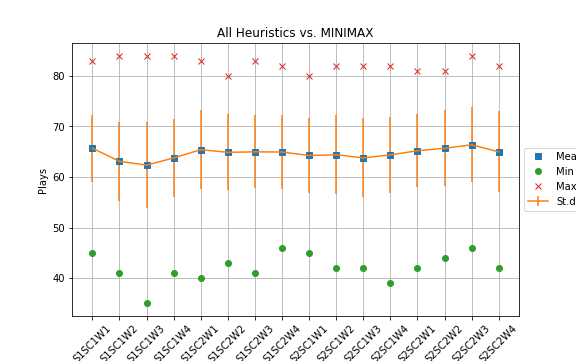
\includegraphics[width=1\columnwidth]{fig/results_Plays_All_vs_MINIMAX.png}
\caption{Plays for all custom heuristics vs. sample player MINIMAX.}
\end{center}
\label{figplyesMINIMAX}
\end{figure}
    

    \begin{table}[htpb]
    \caption{ Plays: all custom heuristics vs. MINIMAX.}
    \centering
    \begin{tabular}{ l | c c c c }
    Heuristic & mean & st.d. & min & max \\ \hline 
    S1SC1W1 & 65.67 & 6.65 & 45.00 & 83.00 \\
    S1SC1W2 & 63.09 & 7.75 & 41.00 & 84.00 \\
    S1SC1W3 & 62.34 & 8.44 & 35.00 & 84.00 \\
    S1SC1W4 & 63.76 & 7.75 & 41.00 & 84.00 \\
    S1SC2W1 & 65.39 & 7.79 & 40.00 & 83.00 \\
    S1SC2W2 & 64.86 & 7.48 & 43.00 & 80.00 \\
    S1SC2W3 & 64.96 & 7.21 & 41.00 & 83.00 \\
    S1SC2W4 & 64.92 & 7.34 & 46.00 & 82.00 \\
    S2SC1W1 & 64.24 & 7.37 & 45.00 & 80.00 \\
    S2SC1W2 & 64.39 & 7.85 & 42.00 & 82.00 \\
    S2SC1W3 & 63.77 & 7.79 & 42.00 & 82.00 \\
    S2SC1W4 & 64.36 & 7.59 & 39.00 & 82.00 \\
    S2SC2W1 & 65.18 & 7.18 & 42.00 & 81.00 \\
    S2SC2W2 & 65.67 & 7.55 & 44.00 & 81.00 \\
    S2SC2W3 & 66.35 & 7.38 & 46.00 & 84.00 \\
    S2SC2W4 & 64.97 & 7.97 & 42.00 & 82.00 
    \end{tabular}
    \label{tabplaysMINIMAX}
    \end{table}

    
%==============================================


\begin{figure}[htpb]
\begin{center}
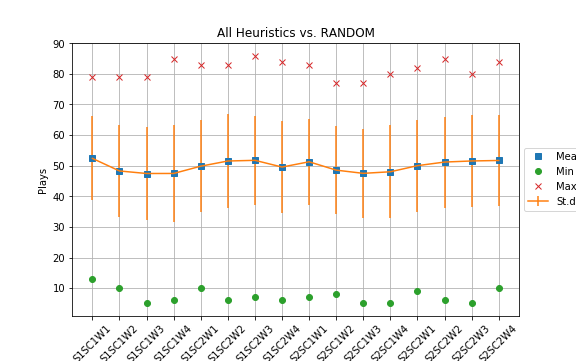
\includegraphics[width=1\columnwidth]{fig/results_Plays_All_vs_RANDOM.png}
\caption{Plays for all custom heuristics vs. sample player RANDOM.}
\end{center}
\label{figplyesRANDOM}
\end{figure}
    

    \begin{table}[htpb]
    \caption{ Plays: all custom heuristics vs. RANDOM.}
    \centering
    \begin{tabular}{ l | c c c c }
    Heuristic & mean & st.d. & min & max \\ \hline 
    S1SC1W1 & 52.38 & 13.70 & 13.00 & 79.00 \\
    S1SC1W2 & 48.28 & 14.98 & 10.00 & 79.00 \\
    S1SC1W3 & 47.45 & 15.10 & 5.00 & 79.00 \\
    S1SC1W4 & 47.47 & 15.89 & 6.00 & 85.00 \\
    S1SC2W1 & 49.84 & 15.06 & 10.00 & 83.00 \\
    S1SC2W2 & 51.53 & 15.23 & 6.00 & 83.00 \\
    S1SC2W3 & 51.76 & 14.56 & 7.00 & 86.00 \\
    S1SC2W4 & 49.56 & 14.95 & 6.00 & 84.00 \\
    S2SC1W1 & 51.28 & 14.12 & 7.00 & 83.00 \\
    S2SC1W2 & 48.55 & 14.39 & 8.00 & 77.00 \\
    S2SC1W3 & 47.50 & 14.64 & 5.00 & 77.00 \\
    S2SC1W4 & 48.02 & 15.12 & 5.00 & 80.00 \\
    S2SC2W1 & 50.02 & 15.05 & 9.00 & 82.00 \\
    S2SC2W2 & 51.19 & 14.86 & 6.00 & 85.00 \\
    S2SC2W3 & 51.55 & 15.11 & 5.00 & 80.00 \\
    S2SC2W4 & 51.71 & 14.89 & 10.00 & 84.00 
    \end{tabular}
    \label{tabplaysRANDOM}
    \end{table}

    
%==============================================


\begin{figure}[htpb]
\begin{center}
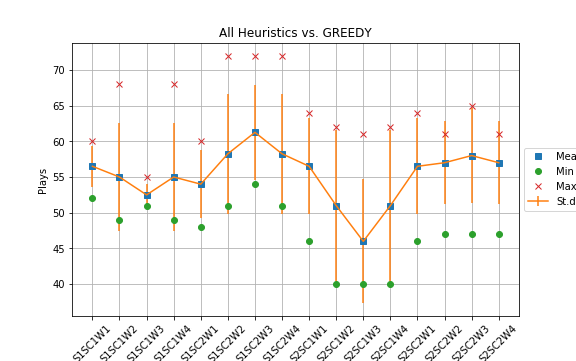
\includegraphics[width=1\columnwidth]{fig/results_Plays_All_vs_GREEDY.png}
\caption{Plays for all custom heuristics vs. sample player GREEDY.}
\end{center}
\label{figplyesGREEDY}
\end{figure}
    

    \begin{table}[htpb]
    \caption{ Plays: all custom heuristics vs. GREEDY.}
    \centering
    \begin{tabular}{ l | c c c c }
    Heuristic & mean & st.d. & min & max \\ \hline 
    S1SC1W1 & 56.50 & 2.87 & 52.00 & 60.00 \\
    S1SC1W2 & 55.00 & 7.58 & 49.00 & 68.00 \\
    S1SC1W3 & 52.50 & 1.50 & 51.00 & 55.00 \\
    S1SC1W4 & 55.00 & 7.58 & 49.00 & 68.00 \\
    S1SC2W1 & 54.00 & 4.74 & 48.00 & 60.00 \\
    S1SC2W2 & 58.25 & 8.38 & 51.00 & 72.00 \\
    S1SC2W3 & 61.25 & 6.68 & 54.00 & 72.00 \\
    S1SC2W4 & 58.25 & 8.38 & 51.00 & 72.00 \\
    S2SC1W1 & 56.50 & 6.69 & 46.00 & 64.00 \\
    S2SC1W2 & 51.00 & 10.51 & 40.00 & 62.00 \\
    S2SC1W3 & 46.00 & 8.69 & 40.00 & 61.00 \\
    S2SC1W4 & 51.00 & 10.51 & 40.00 & 62.00 \\
    S2SC2W1 & 56.50 & 6.69 & 46.00 & 64.00 \\
    S2SC2W2 & 57.00 & 5.79 & 47.00 & 61.00 \\
    S2SC2W3 & 58.00 & 6.67 & 47.00 & 65.00 \\
    S2SC2W4 & 57.00 & 5.79 & 47.00 & 61.00 
    \end{tabular}
    \label{tabplaysGREEDY}
    \end{table}

    
%==============================================


\end{document}